\chapter{Discussion}

\section{Limitations and Improvement}

\subsection{Ranges of Debug Parameters}

In the simulation, the debug parameters were utilized to adjust the locomotion of the quadruped robot. The ranges of debug parameters are given in advance. The fixed ranges would not affect the robot when it performs a single action. Nevertheless, it is not appropriate for the robot to use the fixed range when performing multiple actions at the same time. For example, if the robot stretches its legs to reach the highest squatting position, which means the legs have reached the longest. Afterwards, moving other sliders will lead to program errors, and the robot will disappear in the GUI\cite{ref:GUI} owing to the errors.

To avoid the error caused by the fixed range, the approach is to calculate the real-time debug parameter range according to the joint state of the robot. However, the real-time value ranges need to get the joints' state firstly, then bring them into the correlation matrix to deduce the value range inversely, and compare it with the value range of the joint itself. The complexity of real-time range is close to the quadrupedal locomotion, so it is hard for us to spare time to optimize this part of the code. Otherwise, there is another way to improve the robustness of the code, which is to narrow the range make it so that the robot cannot reach the limit range. Although the problem is not solved from the root, there is less possibility that the code will make mistakes during operation.

\subsection{Non-zero steady-state error}

When the robot is stationary, its joints are not completely static. The robot's joints would move in a minute range. The range of this steady-state error is approximately five decimal places. However, the current state read is used as a reference when controlling the attitude of the robot. Therefore, the previous steady-state error will be substituted into the next action, and the program does not know the generation of this error. In the process of research, we find that as long as the accuracy of the parameters is controlled in three places after the decimal point, the steady-state error can be effectively reduced. But in theory, the problem of steady-state error should not be solved in this way. Therefore, in the following aspects that can be improved, we hope to reduce the steady-state error by using the robust integral controller\cite{ref:RNIcontrol} for the nonlinear system.

\subsection{Friction between the plane and robot}

When dragging the slider rapidlly to adjust the attitude of the robot, the robot will shift from the original position. This is because the friction between the toe joints of the robot and the plane is too small to provide the necessary force for the robot to move under this acceleration. The solution is to increase the friction coefficient between the toe joints and the plane in order to increase the friction force.


\section{Future work}

Due to lack of time, many different adaptations, tests, and experiments are left for the future (the depth of research that can be done in four weeks is limited). Future work can involve in-depth analysis of
the motion mechanism of quadruped robots and try more simulations of actions.
This project mainly focuses on three actions of the quadruped robot, namely pitch angle, yaw angle, and roll angle, and also includes a squat action. The basic theories are basically from robotics and mathematics (geometry and linear algebra), and the following ideas can be tested in future work:

\subsection{New motions}

1. It may be interesting to consider more new motions, such as Z-axis-based bouncing or climbing, depending on deep learning and flexible use of robotics, such as creating new kinematic equations and matrices. For example, using these movements in practice will facilitate movement on more complex terrain. In addition, try to study more complex movements, such as back flips, which Boston Dynamics achieved.

2. Create a new robot model (Unified Robot Description Format): Instead of using an existing open-source model, the robot is described based on the XML syntax framework. ROS provides a C++ interpreter for URDF files, which can parse this kind of robot. format file. Fortunately, although starting from building a model is a tedious task, it is possible to start with what we have learned in the second semester of ELEC230.

\section{Intellectual property}
This project uses the robot model "A1" of Shuyu Technology, which is a patent belonging to their company. It is necessary to declare their patent here: U.S. patent number D916,202 [Application Number D/718,514] was granted by the patent office on 2021-04-13 for quadruped robot. The grantee listed for this patent is HangZhou YuShu TECHNOLOGY CO., LTD.. Invention is credited to Xingxing Wang, Zhiyu Yang.
>>>>>>> Stashed changes

\section{Completion of objectives}

\subsection{Pitching}

When the pitch angle is 0, the body of the robot remains perpendicular to the longitudinal axis perpendicular to the ground. By changing the pitch angle, the front or rear leg of the robot is flexed, while the other leg is extended. What is visually reflected is that the robot is constantly leaning forward and backward with the adjustment of the pitch angle. The simulation of the pitching motion was quite successful.

\subsection{Yawing}

When changing the magnitude of the yaw angle, it can be seen from the direction perpendicular to the body of the robot from below that the legs on the front side of the robot move in opposite directions to the legs on the back side. The body of the robot rotates during yaw. When the yaw angle is positive, the robot body rotates clockwise, and when the yaw angle is negative, the robot body rotates counterclockwise. However, due to the influence of ground friction, the robot will slide when the yaw angle is changed many times, but this does not affect the simulation. The objective for the simulation of yaw motion was also successfully completed.

\subsection{Rolling}

When changing the magnitude of the roll angle, from the front view of the robot, the leg on one side of the robot is extended and the leg on the other side is flexed. The observed scenario is that one side of the robot is raised in height, while the other side is lowered in height. This means that the simulation of the roll motion has been successfully completed.

\subsection{squatting}

As an additional goal of the project, squatting is actually simpler than the other three motions, so the simulation of this action is done first. When we pull the height slider in the program, the four legs of the robot will flex or stretch at the same time, thus completing the adjustment of the body height.

\subsection{Motion combination}

After combining the three simulation programs, an attitude control program that can adjust three angles at the same time is obtained. In Fig.\ref{fig: Combination_of_three_motions}, the first picture is to adjust the roll angle, the second picture is to adjust the pitch angle based on the first picture, and the third picture is to adjust the yaw angle based on the second picture.

\begin{figure}[htbp]
   \centering
   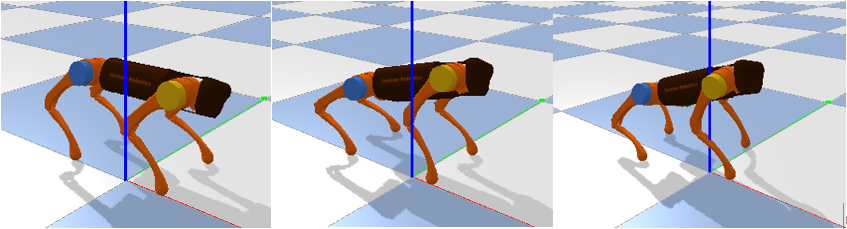
\includegraphics[width=0.8\textwidth]{figures/Combination_of_three_motions.png}
   \caption{Combination of three motions}
   \label{fig: Combination_of_three_motions}
\end{figure}

After combining the attitude adjustment program including three actions with the height adjustment program, the attitude adjustment program with height adjustment function is obtained, which is the final result of this project. The simulation results are shown in Fig.\ref{fig: Pose_control_with_height}. The first picture in Fig.\ref{fig: Pose_control_with_height} is the attitude of the robot after adjusting the pitch angle, yaw angle and roll angle. By adjusting the height, the attitude in the second picture is obtained.

\begin{figure}[htbp]
   \centering
   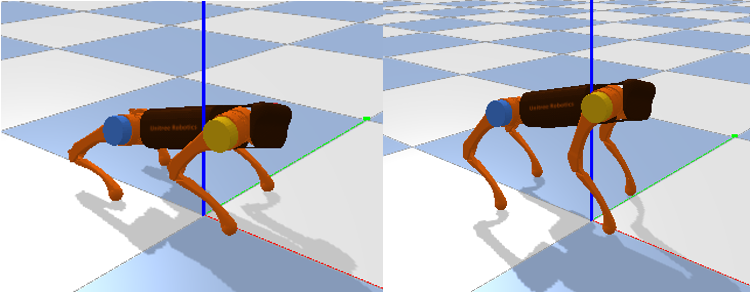
\includegraphics[width=0.8\textwidth]{figures/Pose_control_with_height.png}
   \caption{Pose control with height}
   \label{fig: Pose_control_with_height}
\end{figure}

\chapter{Conclusion}

This report explains the development ideas and final results of the year 2 project. First the project was split into three main motion simulations, pitch, yaw and roll motions and a secondary goal, height adjustment. The ultimate objective is to design a robot attitude control program with height control function. Then we introduced the development environment of the project. Next we explained how to model the legs of a quadruped robot and use trigonometry knowledge and forward and inverse kinematics algorithms to deduce the kinematic model of the quadruped robot legs. After taht we showed the simulation results of height adjustment, pitch, yaw and roll motions respectively. We then discussed this pose control program in terms of limitations and improvement, future work, intellectual property, and completion of objectives. Hope this year 2 project can be helpful to students who choose quadruped robot simulation as their subject in the future.
